%
% Introduction to quantum information theory
%

\section{Introduction to quantum information theory}\index{Quantum information theory}

\famousquote{When you find yourself in a room surrounded by your enemies you tell yourself, `I am not locked in here with you, you are locked in here with me'. This is the kind of mindset you should have if you want to succeed in life. Get rid of that victim mentality.}{Bruce Lee}

% Probability, information & classical correlation measures

\subsection{Probability, information \& classical correlation measures}

``Information theory begins with the observation that there is a fundamental link between probabilities and information.''\comment{Is this a quote? Who?} With any given event (we call this a random variable), associated with such an event is a set of outcomes, each with a certain probability of occurring. 

Suppose we have a random variable $X$, and a particular measurement outcome $x$ occurs with probability $p(x)$, the Shannon entropy\index{Shannon entropy} of $X$ is given by,
\begin{align}
	H(X) = -\sum_x p_x\log_2(p_x).
\end{align}

The information, or entropy, plays a central role in information theory. The intuitive interpretation is that it quantifies an experimenter's uncertainty about $X$ before measuring it, and his expected information gain is $H(X)$ bits upon learning the outcome. The information $H(X)$ is zero if and only if one of the probabilities $p(x)$ is unity, with the others being zero. In this case the value of $X$ is already known and so there is no information to be gained from observing it.  

For a joint distribution over $X$ and $Y$ this generalises to become the joint Shannon entropy\index{Joint Shannon entropy},
\begin{align}
H(X,Y) = -\sum_{x,y} p_{x,y}\log_2(p_{x,y}).
\end{align}

\begin{figure}[!hbtp]
	%\includegraphics[clip=true, width=0.475\textwidth]{classical_mutual_info}
	\captionspacefig \caption{\comment{Missing PDF. To do}}\label{fig:mutual_info}	
\end{figure}

\comment{Should we include Mike and Ike styled Venn diagram for information relationships?}

We now introduce an entropic measure of common or mutual information shared by two parties. Suppose Alice possesses the random variable $A$ and Bob has the random variable $B$, the \textit{mutual information} specifies the number of bits in common between the two distributions. Equivalently, this represents the maximum number of bits that one party can learn about the other just by inspecting their own information.

For two classical distributions, the classical mutual information\index{Mutual information} is given by,
\begin{align}
	I(A;B) = H(A) + H(B) - H(A,B).
\end{align}

It is a measure of the correlation between the events $A$ and $B$. If these correspond, respectively, to the selection and receipts of a signal then \mbox{$H(A:B)$} is the information transferred by the communication. 

The relationship between the quantities mentioned above is graphically summarised in Fig.~\ref{fig:mutual_info}.

% Quantum information

\subsection{Quantum information}

The von Neuman entropy\index{von Neuman entropy} \cite{bib:bengtsson2017geometry} for quantum density operators, $S(\hat\rho)$, is defined analogously, replacing probabilities with density operator eigenvalues,
\begin{align}
S(\hat\rho) &= - \sum_x \lambda_x \log_2 (\lambda_x) \nonumber \\
&= -\mathrm{tr}(\hat\rho\,\log \,\hat\rho),
\end{align}
where $\{\lambda\}$ is the eigenvalue spectrum of $\hat\rho$. This modification is logically justified, as the eigenvalues can be interpreted directly as a purely classical probability distribution of orthogonal states when the density operator is transformed into a basis with no coherences between basis states (i.e a diagonal basis or spectral decomposition\index{Spectral decomposition}). In that case, the Shannon and von Neuman entropies essentially have identical physical interpretations.

Analogously, the quantum mutual information\index{Quantum mutual information} for bipartite state $\hat\rho_{A,B}$ is defined as,
\begin{align}
I(A;B)_{\hat\rho} = S(\hat\rho_A) + S(\hat\rho_B) - S(\hat\rho_{A,B}),
\end{align}
using the von Neuman entropy.

The mutual information between two quantum states is invariant under local unitary transformations,
\begin{align}
I(A;B)_{\hat\rho} = I(\hat{U}_A\hat\rho_A \hat{U}_A^\dag; \hat{U}_B\hat\rho_B \hat{U}_B^\dag),
\end{align}
since the eigenvalue spectrum of a density operator is invariant under unitary transformations. Therefore, the mutual information represents the maximum amount of information Bob can learn about Alice's state under \textit{any} local operations.

A quantum process (the most general form of quantum evolution, described in Sec.~\ref{sec:quantum_processes}) cannot increase the mutual information between two parties. This yields the \textit{data processing inequality}\index{Data processing inequality} that, for a sequence of channels \mbox{$X\to Y\to Z$},
\begin{align}\index{Data processing inequality}\label{eq:data_proc_ineq}
	I(X:Z)&\leq I(X:Y), \nonumber \\
	I(X:Z)&\leq I(Y:Z),
\end{align}
with equality if and only if the channel not specified in the identity on the right hand side (\mbox{$Y\to Z$} or \mbox{$X\to Y$} respectively) is unitary, i.e one of the links in the chain perfectly preserves information content. The progression is shown in Fig.~\ref{fig:data_proc_ineq}.

\begin{figure}[!htbp]
	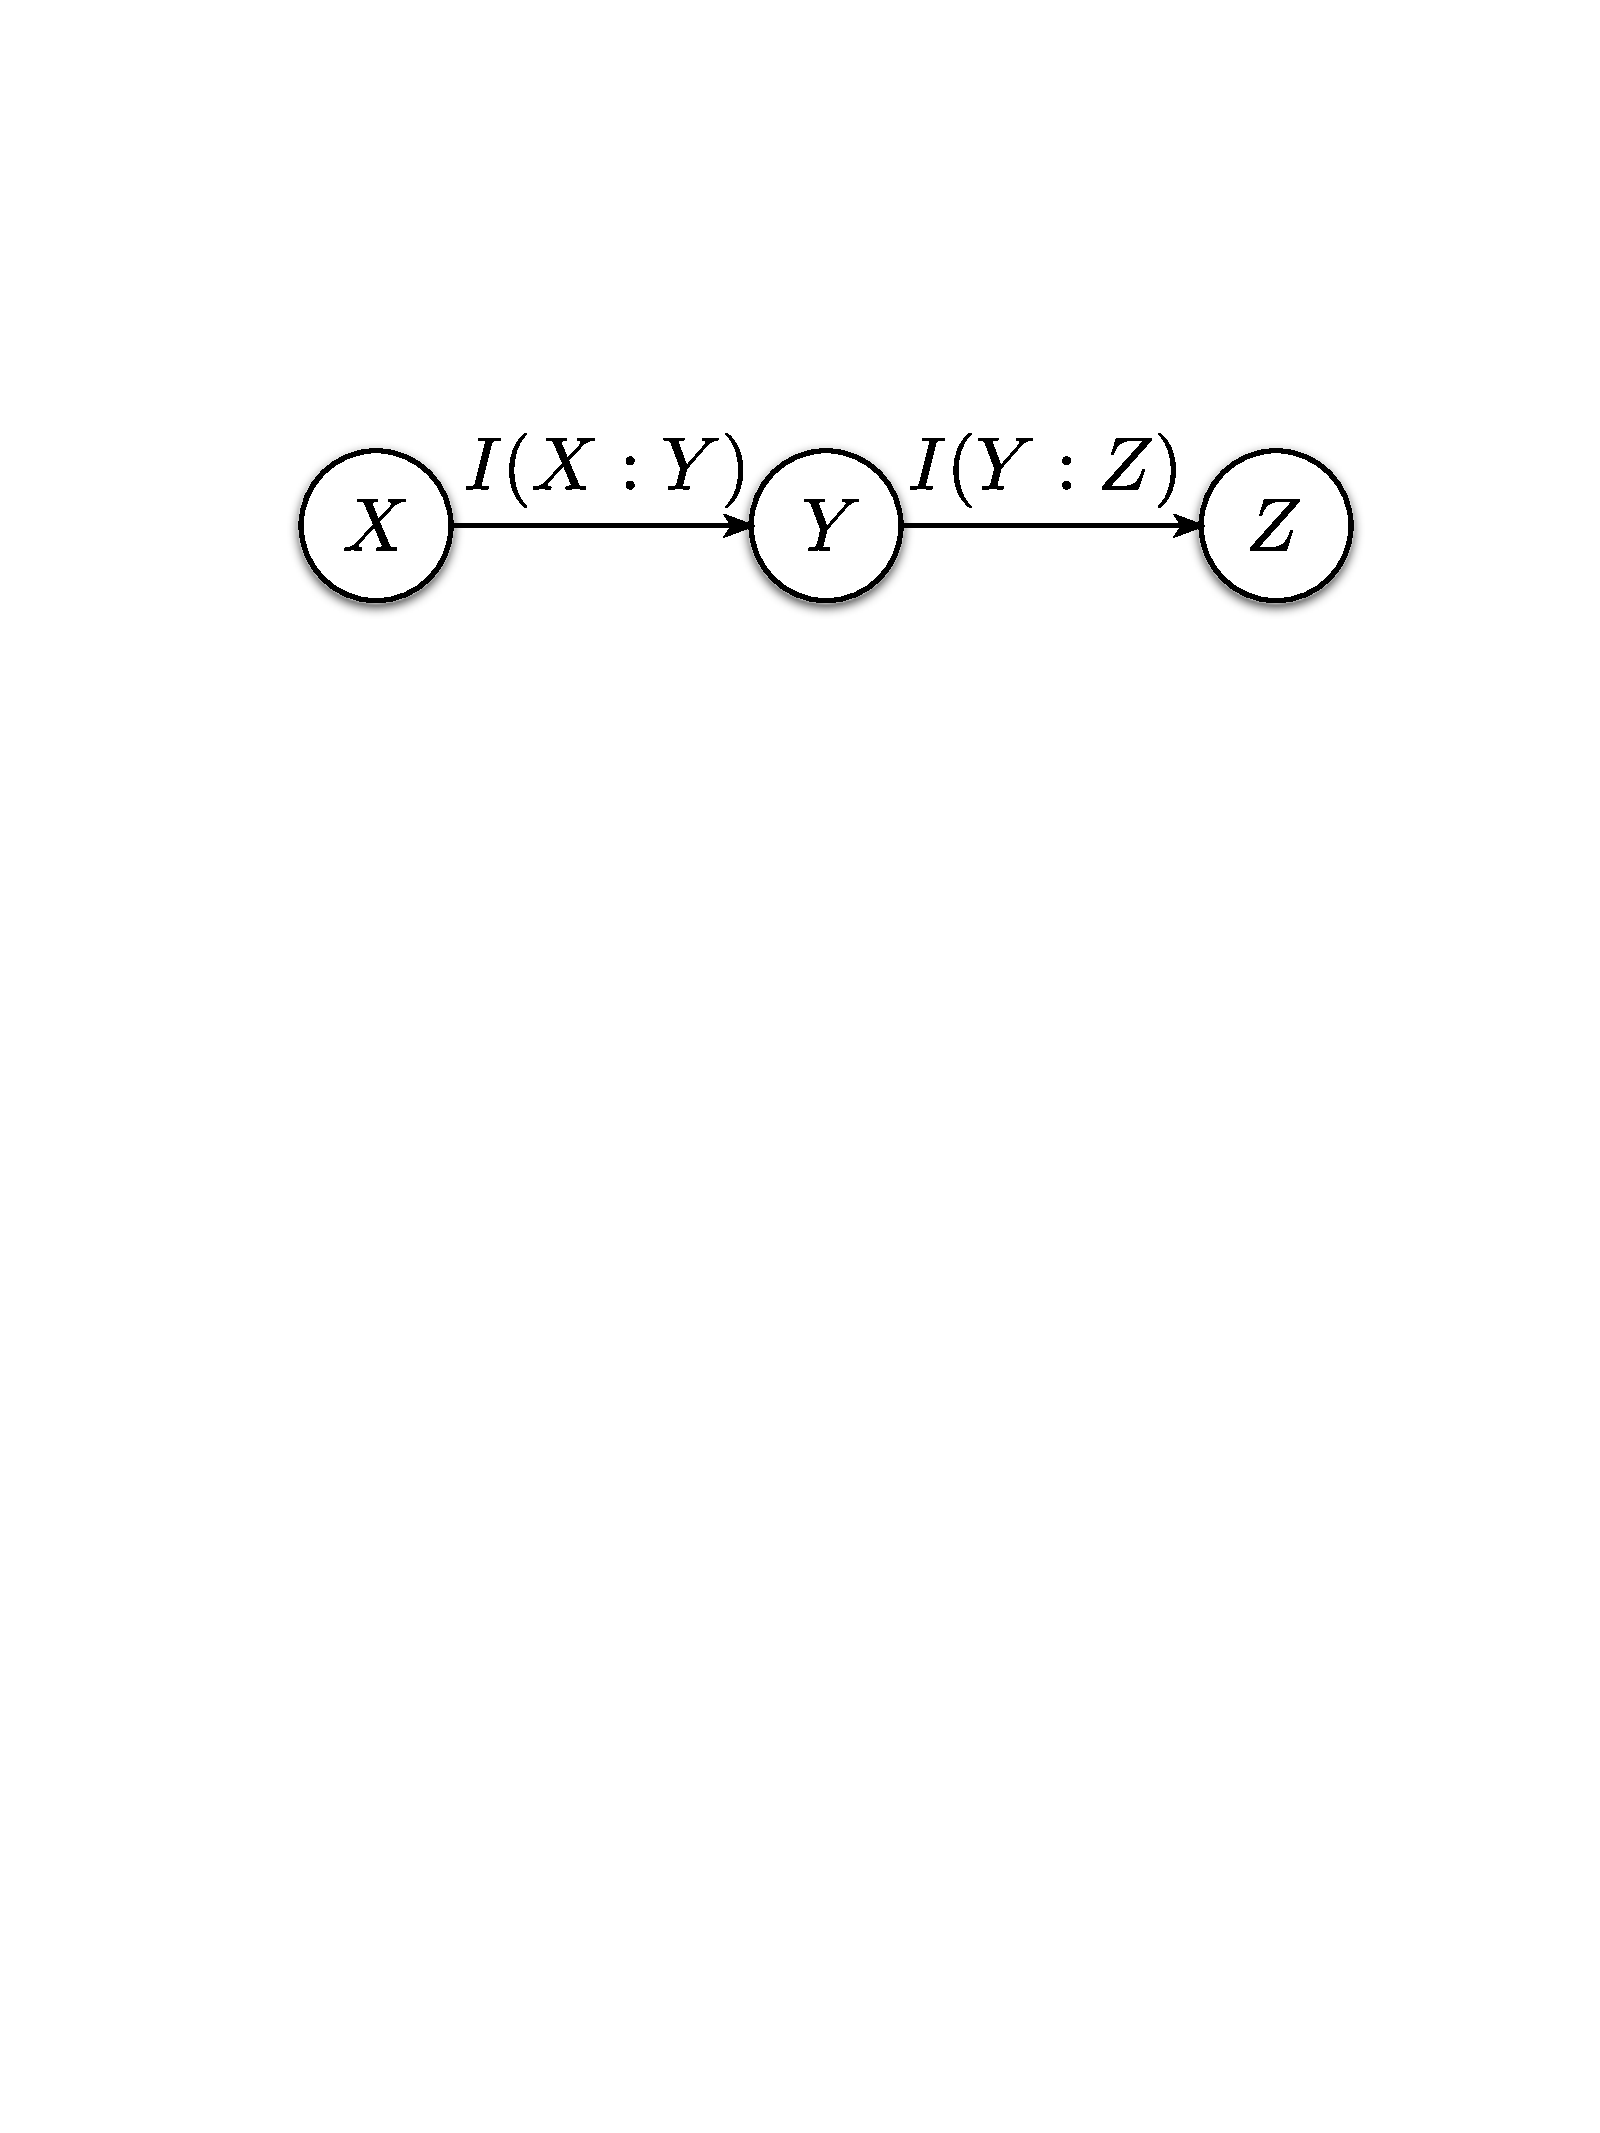
\includegraphics[clip=true, width=0.3\textwidth]{data_proc_ineq}
	\captionspacefig \caption{\label{fig:data_proc_ineq}A sequence of events \mbox{$X\to Y\to Z$}. The data processing inequality states that the mutual information from beginning to end is upper-bounded by the mutual information between neighbouring stages, as per Eq.~(\ref{eq:data_proc_ineq}).}	
\end{figure}

The mutual information is defined as being between a particular known pair of states. Of course, in a quantum channel we have the flexibility to manipulate the input state and the measurement at the output. From this, we can then define the \textit{classical information of the channel}\index{Classical information of the channel}, $I_c(\hat\rho_{A,B})$ -- the maximum of the mutual information, optimised over \textit{all} possible measurement settings. Suppose $\hat\rho_{A,B}$ is shared between Alice and Bob, from which they would like to extract maximal correlations (i.e joint information). They measure using local measurement bases $\{\Lambda_A^x\}$ and $\{\Lambda_B^x\}$, yielding random variables $A$ and $B$. Their quantum mutual information of the channel is defined as,
\begin{align}
I_c(\hat\rho_{A,B}) = \max_{\rho,\{\Lambda_A^x\},\{\Lambda_B^x\}} I(A;B). \label{eq:quant_mut}
\end{align}

The intuitive interpretation is that this is the maximum mutual information between input and output states that can be achieved across the channel. This effectively places a physical upper bound on the achievable bitrate or bandwidth of the channel.

% Quantum correlation measures

\subsection{Quantum correlation measures}

We now move on to discuss quantum correlations. Whilst classical correlation measures have a clear operational meaning, quantum channel capacities are less so -- these quantities can be interpreted as how well the channel preserves the quantum state.

Analogous to the mutual information for classical systems is the \textit{coherent information}\index{Coherent information} for quantum systems \cite{bib:PhysRevA.54.2629}, defined as,
\begin{align}\label{eq:mutual_info_classical_single}
I(\hat\rho,\mathcal{E}) = S(\mathcal{E}(\hat\rho)) - S_e(\hat\rho,\mathcal{E}).
\end{align}
Here $S_e$ is the \textit{exchange entropy}, a measure of how much information is exchanged between the state $\hat\rho$ and the environment under the action of the process. Specifically, it is given by the entropy of the environment subsystem in Eq.~(\ref{eq:proc_environment}), after application of the channel. This yields the intuitive interpretation that the coherent information is the information contained in the evolved state, discounted by the amount lost to the environment. It can be alternatively written as,
\begin{align}
I(A\rangle B) = H(B)_{\hat\rho} - H(A,B)_{\hat\rho},
\end{align}
which we recognise as the negative of the \textit{conditional quantum entropy}\index{Conditional quantum entropy},
\begin{align}
H(A|B) = H(A,B)_{\hat\rho} - H(B).
\end{align}
The fact that the information quantity $H(A|B)$ can be negative is a signature of the fundamental difference between the laws of classical and quantum information.

The quantum coherent information exhibits much of the same mathematical structure as the classical mutual information. And analogously,
\begin{align}\index{Quantum channels!Capacity}
\mathcal{I}_Q(\mathcal{E}) = \max_{\hat\rho} I(\hat\rho,\mathcal{E}).
\label{eq:mutual_info_quantum_single}
\end{align}